\chapter{Movie Data Processing and Success Prediction}
\label{chapter:model}
This chapter presents the methodology necessary to predict movie success and a
characterization of the dataset. We start by describing the steps for
filtering, processing and interpreting the dataset along with characterizations
in Section~\ref{sec:dataset_interpret}. Then, we present our new methodology to
correctly interpret the dataset into movie parameters suitable for analysis in
a prediction model in Section~\ref{sec:features}–this includes movie success
parameters and social parameters from movie-producing teams. In
Section~\ref{sec:feature_char}, we characterize the dataset in terms of such
parameters. In Section~\ref{sec:feature_interac}, we discuss feature
interaction. Finally, in Section~\ref{sec:model:prediction}, we present and
describe the prediction model and methodology employed to assess how movie
characteristics are related to movie success.

\section{Dataset Processing}
\label{sec:dataset_interpret}
This section presents all pre-processing steps necessary to extract the proper
information required for our analysis. We present the network model and 
strategies for filtering irrelevant information from the dataset, as well as
extracting and normalizing movie success parameters. We then group the movies
into three performance groups and present a characterization for the adjusted
success parameters and performance groups.

\subsection{Network Model}
Assessing topological information from movie production teams requires to build
a graph for modeling the interaction network of movie producing agents as
accurately as possible. Specifically, we construct a graph for movie producers
only, leaving out the rest of the crew and cast (actors, directors, writers,
etc.). The reason is that producers are the \textit{core} of the team: they
make the most important decisions and hire the rest of the crew, ultimately
claiming most responsibility for the success of the movie.  Furthermore, adding
more types of agents to the model would make it orders of magnitude larger,
exceeding the computing power available and possibly adding uncertainty to the
results~\citep{COSN2014-cost1,elberse2007power,COSN2014-cost2}.

As discussed in Section~\ref{sec:fundamentals:social}, most
network measures are only defined for one-mode networks, so our network model
cannot be directly based on a bipartite network. As presented in
Section~\ref{sec:foundamentals:dataset}, IMDb provides co-production data from
movies that is directly mappable to a bipartite collaboration network.
Therefore, one initial step in pre-processing the IMDb dataset is to derive an
one-mode network from it. To this end, we employ the methodology proposed
by~\cite{newman2001scientific}.

Formally, given a set of movies $\mathbb{M}$, each movie $m \in \mathbb{M}$ has
a set of producers $\mathbb{P}_m$ (also called $m$'s production team). All
producers $p \in \mathbb{P}_m$ are connected nodes in a graph
$\mathbb{G}_\mathbb{P}$, which aggregates all producers of all movies in
$\mathbb{M}$. Moreover, edges in $\mathbb{G}_\mathbb{P}$ are undirected and
link producers who have worked together in one or more movie. The number of
previous collaborations between two producers is expressed by a weight value in
the edge connecting them. For every node $p$, $H_p$ is $p$'s past experience
(i.e.\@ the number of $p$'s previous productions), and $S_p$ is $p$'s previous
success (i.e.\@ the mean of success parameters for $p$'s movies). Finally,
$\mathbb{G}_\mathbb{P}$ evolves over time to incorporate new data when new
movies are produced. Therefore, $\mathbb{G}_\mathbb{P}(t)$ represents the
connections among producers considering only movies that were released up to
instant $t$.

For any given movie $m$, its characteristics are based on the topology from the
subset of nodes in $\mathbb{P}_m$. For assessing $m$'s characteristics, the
graph is set to the state of the movie's release date; hence, whatever happened
after the movie's production does not affect its features. This is achieved by
processing movies in chronological order. By doing so, once a movie is
processed, the graph only contains information from the already processed,
previously released movies.

Besides edges and nodes, an auxiliary data structure is annexed to $\mathbb{G}$
to accommodate necessary non-topological information from movies. As presented
in Section~\ref{sec:foundamentals:dataset}, the IMDb dataset provides an
incredibly rich pool of information, including collaboration data from
producing agents. Some of this auxiliary, pre-release information is extracted
from the dataset and stored separately from the graph: movie budget (adjusted
and normalized as is movie gross), movie duration in minutes, genre (such as
Action, Drama, Sci-Fi, etc.) and production countries. This information is also
used by~\cite{Ghiassi2015} in their pre-release movie success prediction
analysis.

With such a model, we are able to represent the entire producing network from
IMDb in a graph. However, because processing power is limited, we need to focus
on those movies whose analysis will potentially produce more significant
results.

\subsection{Dataset Filtering}
\label{sec:filter}
Building a graph for the entire IMDb dataset is very costly and would include
all kinds, shapes and sizes of movies. In order to get more significant results
with minimum noise (i.e.\@ minimum outliers and irrelevant data), we prune some
nodes and their edges. Moreover, it is important to improve the accuracy of our
graph model in representing how movie production parties interact, even if
information must be removed from the graph. Data is filtered before the
experiments according to the following parameters.

\begin{description}
\item [Producer Current Activity.] According to~\cite{uzzi2005collaboration},
once a producer has not worked for seven consecutive years, his/her node should
be removed (we note that such person is likely to be retired or deceased).
\item [Movie Release Date.] The movie industry only cemented itself with the
establishment of the first Academy Awards
(1929)~\citep{bakker2008entertainment}. At that time, sound technology for
movies emerged, people begun to consider movie theaters as an entertainment
option, and professional movie production took off. Considering this, we split
the dataset in 1930: movies released in [1888--1929] are used to bootstrap the
graph creation with starting nodes and edges, and movies released from 1930 on
are considered for our analysis. We note that evaluating social metrics on a
network with very few nodes and edges may produce distorted
results~\citep{newman2010networks}.  Therefore, using early movies to create a
starting graph generates a well defined network in order to properly analyze
the movies from 1930 onwards.  Movies from 2014 on are disregarded because they
were very recently added to the database, and therefore might contain
unreliable (i.e.\@ unstable) key information for the analysis, such as ratings or
gross.
\item [Type of Movie.] We focus on feature-length movies (at least 40 minutes
long\footnote{In order to be eligible for receiving an award from the Academy
of Motion Picture Arts and Sciences (\url{http://www.oscars.org/}), a movie
must fit their definition of ``feature-length'', then having 40 or more minutes
of total runtime.}) produced for cinema. This includes documentaries, but
leaves out TV productions and short movies as they present different goals and
styles.  It is also debatable if their ratings and gross can be compared to
results obtained in the cinema. Over 238,000 movie titles were collected,
involving over 1.7 million different people, of which 246 thousand are
producers.
\item [Relevance.] We are not interested in evaluating amateur productions,
but professionally produced movies (see
Section~\ref{sec:foundamentals:dataset}). Therefore, only movies with at least
1,000 \textit{votes} are considered. Thus, the dataset was reduced to 19,448
titles (about 8.5\% of IMDb) and 39,808 producers\footnote{We have also
analyzed a dataset for movies with at least 100 votes (65,493 titles
representing 28\% of IMDb, and 92,128 producers). Not all network
metrics were computable with such a large dataset, but we were able to identify
similar results for those that finished processing.}.
\item [Team Size and Connectivity.] Movies with just one producer (which does
not characterize a team) or whose producers are not part of the network giant
component are discarded. The final dataset contains 12,250 movie titles with
31,696 producers\footnote{The final dataset is available here:
\url{http://goo.gl/0BPffy}}, as collected in November, 2014.
\end{description}

\subsection{Movie Success Parameters}
\label{sec:success}
As discussed in Chapter~\ref{chapter:intro}, there is no single definition for
movie success. Therefore, we have evaluated the data available at IMDb and
decided to consider three different measures as \textit{success parameters}.
First, \textit{economic success} is given by the gross income, which is
directly connected with the revenue and represents how many people were
interested in paying to watch the movie. Second, \textit{public acceptance} is
given by the IMDb user ratings and indicates how well the title was received by
the general public.  Finally, \textit{movie popularity} is given by the
absolute number of votes the movie received and represents the number of people
who have watched the movie and were interested in evaluating it.

Figure~\ref{fig:scatter_success_params} illustrates the correlation between
these three variables. Note that the relationship presented in
Figure~\ref{fig:scatter_success_params}$(a)$ between \textit{economic success}
and \textit{popularity} confirms the positive correlation found
by~\cite{wasserman2015cross} for these parameters.
Figure~\ref{fig:scatter_success_params}$(b)$ presents the relationship between
movie's \textit{public acceptance} and \textit{popularity}. Note that this
graph has a logarithm scale. Most movies have average
\textit{public acceptance} levels paired with low \textit{popularity}, and
movies in the higher spectrum of \textit{popularity} have an above average
\textit{public acceptance}.  Figure~\ref{fig:scatter_success_params}$(c)$
presents the relationship between movie's \textit{public acceptance} and
\textit{economic success}. It clearly shows that movies with a higher
\textit{economic success} tend to deviate more from the average in terms of
\textit{public acceptance}.

\begin{figure}[tb]\begin{center} %4.1
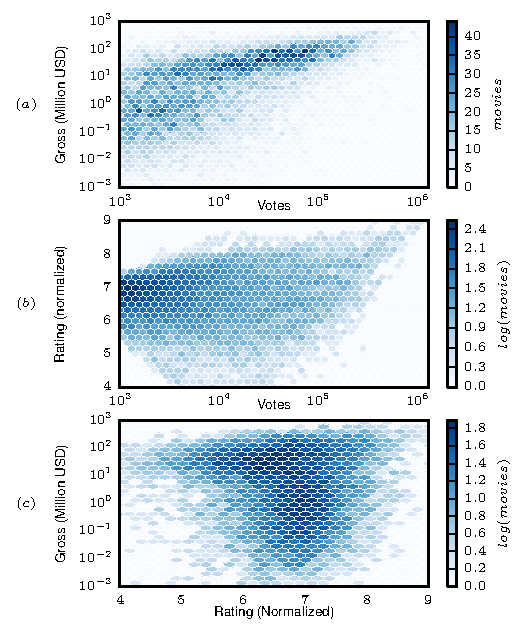
\includegraphics[width=0.85\columnwidth]{../../images/scatter_success_params.pdf}
\caption{\label{fig:scatter_success_params}Relationships between movie's
success parameters}
\end{center}\end{figure}

Since movie \textit{popularity} is positively correlated with \textit{economic
success}, and popular movies have \textit{public acceptance} values that
deviate more from the average (as shown
Figure~\ref{fig:scatter_success_params}$(a)$ and $(b)$), we conclude that all
three graphs are in accordance to each other. Movies with a higher economic
success draw more attention, and therefore have a more diverse pool of opinions
and evaluations. This translates to more heterogeneous values of \textit{public
acceptance}.

Next, we discuss strategies for normalizing each of such success parameter.

\subsubsection{Average Rating}
The trust on the values for average rating increases for movies that received
more ratings (more votes), because a small number of biased evaluations can
significantly change the movie's overall evaluation. Very popular movies have
dozens of thousands of votes, and thus the bias generated by unfair evaluations
is reduced. Therefore, average ratings for popular movies cannot be directly
compared to those of movies that received only a few thousand or even less
evaluations. Hence, average ratings were normalized by the number of votes
received on the same true Bayesian estimate~\cite{bolstad2013introduction} used
by IMDb in its TOP 250 list\footnote{IMDb Top 250
Movies: \url{http://www.imdb.com/chart/top}}, according to the following
equation:

\begin{equation}
\textrm{Weighted Rating} = \left(\frac{v}{v+t_v}\right) \cdot R + \left(\frac{t_v}{v+t_v}\right) \cdot C,
\label{eq:wrating}
\end{equation}
where for each movie, $R$ is the mean of its ratings, $v$ is the number of
votes it received, $t_v$ is a threshold equal to the least amount of votes of a
fully trustable rating, and $C$ is the mean vote across all movies. The value
of $C$ is provided by IMDb\footnote{IMDb
Charts:~\url{http://www.imdb.com/chart/top}} and was equal to $7.0$ at the time
the dataset was collected (November, 2014). A value of $t_v=2,500$ was chosen
in order to ensure log-normal rating distribution (as seen in
Figure~\ref{fig:hist_success}$(c)$). This ensures that movies with few
evaluations (and therefore less trustable mean ratings) have their mean ratings
pushed towards the global mean vote, effectively compensating for the higher
probability of the movie having a biased deviation from the mean that is not
due to the movie itself. For instance, there are several obscure productions
with only a few hundreds of evaluations that have a mean rating that is as high
as the most widely acclaimed movies. However, its unlikely that these movies
have the same level of public acceptance.

\begin{figure}[tb]\begin{center}
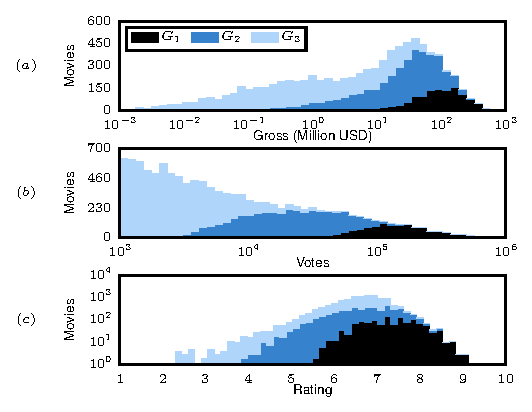
\includegraphics[width=0.85\columnwidth]{../../images/hist_success.pdf}
\caption{\label{fig:hist_success}Histogram of movies per success parameter
aggregated as the three performance groups.}
\end{center}\end{figure}

\subsubsection{Gross Income}
Gross income information was only available for 70\% of movies (9,210
instances). Also, the monetary values are usually given in the currency of the
country that hosted the movie production, and is dated from shortly after the
movie's release. To compare monetary values with minimal distortion, the values
were normalized. Values for gross income and budget were converted to US
Dollars using the Historical Currency Converter Web Service\footnote{Historical
Currency Converter:~\url{http://currencies.apps.grandtrunk.net}}.

Since the dataset contains movies produced in many different decades, US dollar
gross values from distinct moments in history cannot be fairly compared due to
inflation. Therefore, the amounts in US Dollars were subsequently corrected for
inflation using the CPI Inflation Calculator\footnote{CPI Inflation
Calculator:~\url{http://www.bls.gov/data/inflation\_calculator.htm}}, an online
feature provided by the Bureau of Labor Statistics, in October 2014.

The movies without a valid historical exchange record for US Dollars (only six
instances) had their gross information discarded. Movies without gross
information are not considered for analyses involving gross. Finally,
Figure~\ref{fig:hist_success}$(a)$ shows the movies' distribution of gross
income, which follows the shape of a double-normal distribution.

\subsubsection{Number of Votes}
Figure~\ref{fig:hist_success}$(b)$ shows the number of votes a movie
receives follows a power law, spanning several orders of magnitude. For this
reason, these numbers were logarithmically adjusted by following the methodology
proposed by~\cite{ASI:ASI23213}. This adjustment is made because several
regression models are impaired when predicting data that spans several
orders of magnitude.

\subsection{Dataset Characterization}
We now present the distribution of the extracted success features from movies
through decades. Figure~\ref{fig:boxplot_success}$(a)$ shows the histogram of
movie productions throughout the decades. It clearly shows the number of movie
productions exploded in the last decades (note that its y-axis is in
log-scale). We also observe a few changes in the historical distributions of
movie's success parameters.

There have been more movies with inferior box office in recent years
(Figure~\ref{fig:boxplot_success}$(b)$). We argue that, in the past, movie
productions were more expensive to fund and few people could afford a
commercial movie production.  Now, it is cheaper to produce a movie and to sell
it to a specific (niche) audience. Such movies can accumulate a smaller gross
but still be able to cover its production budget. 

In recent decades, movies have more votes
(Figure~\ref{fig:boxplot_success}$(c)$). Also regarding movie's ratings,
Figure~\ref{fig:boxplot_success}$(d)$ shows clearly that older movies have
significantly higher average ratings than recent movies. Ratings are also more
heterogeneous: when compared to the mean value, their ratings are more
dispersed than in previous decades.

We argue that this phenomenon is not due strictly to movies produced in the
past having a higher quality, but also to selection bias. People either choose
a new movie to watch or an old classic with good references: there is little
(or no) motivation to watch unimportant or unsuccessful movies from the past.
It is expected that only good movies from the past are watched and voted on
today.  Furthermore, the IMDb website started collecting ratings from movies in
the nineties. Movies released before that have ratings that are subject to this
selection bias. 

\begin{figure}[tb]\begin{center}
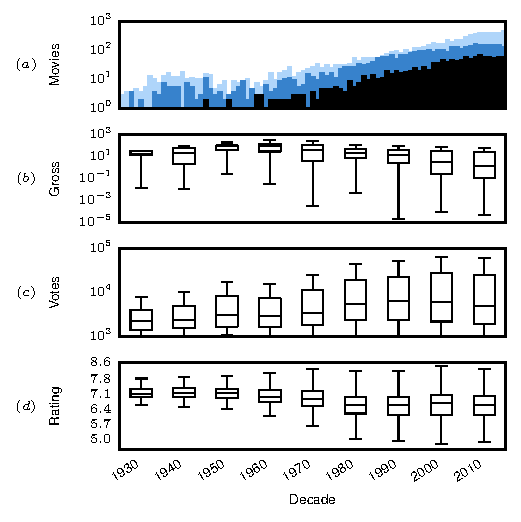
\includegraphics[width=0.85\columnwidth]{../../images/boxplot_success.pdf}
\caption{\label{fig:boxplot_success}Movie productions and their success
parameters through the decades.}
\end{center}\end{figure}

This selection bias also happens because people are constantly motivated by
heavy ad campaigns to watch newer movies, even if they are unsure whether the
movie is worth watching.

\subsection{Movie Grouping by Performance}
For better understanding and analyzing the different degrees of movie success,
we scale the normalized values from the three success parameters (number of
votes, gross income and average rating) in the $[0, 1]$ interval. Subsequently,
we calculate the simple mean of (the scaled values of) their three success
parameters. Then, we take the resulting value and divide the movies that were
considered for the experiment by breaking the distribution into 10 slices (each
slice contains movies whose average mean success falls into one specific
range\footnote{We reaffirm that only movies that pass all constraints defined
in Section~\ref{sec:filter} take part in this analysis.}). For example, slice
0--10\%  contains the top 10\% most successful movies, while slice 10--20\%
contains movies whose success parameter values fall between the
10\textsuperscript{th} and 20\textsuperscript{th} percentile of the success
distribution. Table~\ref{tab:success_groups} shows the number of movies and the
total number of movies per slice as well. Overall, we aggregate the slices into
three major groups: group $G_1$ with blockbusters, group $G_2$ with movies of
moderate success, and group $G_3$ with movies of low success.

\begin{table}[tb]
\caption{\label{tab:success_groups} Grouped distribution of success.}
\centering
\begin{tabular}{@{}llllllc@{}}
\toprule
Slice    & \xcell{\# of\\Movies} & \xcell{Mean\\Success} & \xcell{Mean\\Rating} & \xcell{Mean\\Gross} & \xcell{Mean\\Votes} & Group\\ \midrule
0--10\%   & 1225  & 0.764       & 0.738    & 0.865   & 0.690   & $G_1$                  \\ \midrule
10--20\%  & 1225  & 0.665       & 0.663    & 0.808   & 0.523   & \multirow{3}{*}{$G_2$} \\
20--30\%  & 1225  & 0.607       & 0.647    & 0.766   & 0.409   &                     \\
30--40\%  & 1225  & 0.563       & 0.638    & 0.735   & 0.315   &                     \\ \midrule
40--50\%  & 1225  & 0.529       & 0.641    & 0.704   & 0.243   & \multirow{6}{*}{$G_3$} \\
50--60\%  & 1225  & 0.506       & 0.644    & 0.687   & 0.186   &                     \\
60--70\%  & 1225  & 0.485       & 0.649    & 0.676   & 0.131   &                     \\
70--80\%  & 1225  & 0.468       & 0.638    & 0.665   & 0.100   &                     \\
80--90\%  & 1225  & 0.447       & 0.610    & 0.628   & 0.102   &                     \\
90--100\% & 1225  & 0.394       & 0.599    & 0.482   & 0.101   &                     \\ \midrule
\end{tabular}
\end{table}


Going back to Figure~\ref{fig:hist_success}, it shows the distribution of the
number of movies with respect to the success parameters after normalization.
Their distributions are drastically different among the tree groups, specially
regarding gross (Figure~\ref{fig:hist_success}$(a)$) and number of votes
(Figure~\ref{fig:hist_success}$(b)$). In Chapter~\ref{chapter:analysis}, we
further discuss the different characteristics among these groups.
  % this is how we interpret the dataset.
\section{Defining Features for Movies}
\label{sec:features}

This section presents the features extracted from each movie, which can be
divided into two main groups: features related to characteristics from the
movie producing team and features related to the movie itself.
Table~\ref{tab:features} presents an overview of all features.

\begin{table}[h]
\caption{\label{tab:features}All 121 features considered in the experiment.}

\begin{subtable}[b]{\textwidth}
\caption{\textbf{Features obtained via aggregation}}
\centering
\begin{tabular}{@{}llcc@{}} \toprule
Feature Type & Metric Name & \xcell{Number of\\Aggregations} & \xcell{ Number of\\ Features} \\ \midrule
\multirow{10}{*}{\xcell{Ego\\Metrics}} & Closeness  & 7 & \multirow{10}{*}{70}    \\
        & Betweenness  &  7  &         \\
        & Clustering   & 7   &         \\
        & Square clustering & 7 &      \\
        & Degree                     & 7                          &                         \\
                        & Net.\ constraint           & 7                          &                         \\
                        & Prev.\ rating              & 7                          &                         \\
                        & Prev.\ gross               & 7                          &                         \\
                        & Prev.\ votes               & 7                          &                         \\
                        & Prev.\ experience          & 7                          &                         \\ \midrule
\multirow{3}{*}{\xcell{Pairwise\\Metrics}} & Past experience            & 6                          & \multirow{3}{*}{18}     \\
                        & Shared friends             & 6                          &                         \\
                        & Neighbour overlap          & 6                          &                         \\ \bottomrule
\end{tabular}
\end{subtable}

\vspace{6pt}

\begin{subtable}[b]{\textwidth}
\caption{\textbf{Features obtained via One-Hot Encoding}}
\centering
\begin{tabular}{@{}llcc@{}} \toprule
Feature Type             & Characteristic                & \xcell{Number of\\Groups}   & \xcell{Number of\\Features}          \\ \midrule
\multirow{2}{*}{\xcell{Movie\\Characteristics}}  & Genres                     & 21                         & \multirow{2}{*}{27}     \\
                        & Continents                 & 6                          &                         \\ \bottomrule
\end{tabular}
\end{subtable}

\vspace{6pt}

\begin{subtable}[b]{\textwidth}
\caption{\textbf{Simple Features}}
\centering
\begin{tabular}{@{}llcc@{}} \toprule
Feature Type             & \multicolumn{2}{l}{Feature Name}                          & \xcell{Number of\\Features}           \\ \midrule
\multirow{3}{*}{\xcell{Global\\Metrics}} & \multicolumn{2}{l}{Global clustering coefficient}                    & \multirow{3}{*}{3}      \\
                        & \multicolumn{2}{l}{Average path length}                          &                         \\
                        & \multicolumn{2}{l}{Small world coefficient}                          &                         \\ \midrule
\multirow{3}{*}{\xcell{Movie\\Characteristics}}   & \multicolumn{2}{l}{Runtime in minutes}    &    \multirow{3}{*}{3}   \\
    & \multicolumn{2}{l}{Production team size}  &            \\
    & \multicolumn{2}{l}{Production budget (normalized)}  &    \\
\bottomrule
\end{tabular}
\end{subtable}
\end{table}


\subsection{From Movie Characteristics}
We include 32 features that are unrelated to social characteristics from the
movie production team composition: the movie's genres, production countries,
runtime length, and the global state of the interaction graph model
(Section~\ref{sec:fundamentals:social}) at the time of the movie's release.
These characteristics have also been previously explored to predict movie
success~\citep{Ghiassi2015} and influence~\citep{wasserman2015cross}.  Next, we
describe the methodology for extracting these features.

Movie genre is categorical data: the IMDb dataset may assign one or more genres
to movies. Therefore, we used 21 binary features to represent this categorical
data, each one representing whether the movie belongs to a specific genre.

The IMDb dataset also provides a list of countries associated with the
production of a movie. Since there are about 200 different countries, it is not
efficient to encode country production into features directly. Therefore, the
UN list for countries and continents was used to transform the movie's list of
related countries into this list of related ``geographic regions'': Africa,
Asia, Europe, Latin America, North America and Oceania. Again, binary features
were used, each encoding whether any country of the given continent took part
in producing the movie. We note that movies can be jointly produced by teams in
different countries, or by teams residing in a single country.

Runtime length and production team size are directly represented as integer
features. Runtimes range from 40 minutes to 450
minutes\footnote{``S\'at\'antang\'o'' by B\'ela Tarr (1994) has a runtime of
432 minutes.}. Production team sizes range from 2 to 19\footnote{Production
team of ``Knuckleball!'' (2012).}.

Finally, we calculate topological characteristics concerning the state of the
whole network (following~\cite{uzzi2005collaboration}): its clustering
coefficient, the average path length, and its small world coefficient.

\subsection{From Movie Production Teams}
Here, we present features derived from the set of social characteristics and
past history from movie producing teams, which are based on the aspects
presented in Table~\ref{tab:team_metrics}. In addition to each producer's track
record, the table contains well known topological metrics regarding social
network analysis, which capture different social aspects of nodes in a social
network graph.

We consider six topological ego-metrics (closeness, betweenness, clustering,
square clustering, degree, and network constraint) and two pairwise-metrics
(shared friends and neighbor overlap). These metrics are defined for singular
nodes or pairs of nodes, and there is no standard methodology for extracting
such topological information from sets of two or more nodes that constitute a
team. To address this problem, we aggregate topological information from nodes
in teams in two different ways: (\textit{i}) we aggregate values from metrics
calculated from single nodes (or pairs of nodes) in the team, and (\textit{ii})
we temporarily contract all nodes from the team into a single node (using node
contraction, Chapter~\ref{sec:fundamentals:social}) and calculate metrics in
the contracted node\footnote{Node contraction cannot be used with pair-wise
metrics, since it aggregates all information into a single node}.

In the first approach, aggregating the different metric values in a single way
(e.g., considering only the simple mean of the values) is prone to information
loss, since many distinct distributions can have the same mean value.
Therefore, in addition to the mean, five other statistical aggregation
functions are used. This way, more information about the distribution of the
values is preserved. The seven methods for statistical and non-statistical
aggregation are briefly presented in Table~\ref{tab:agg}.

Moreover, we consider three global metrics to get the network state at time of
movie release: the global clustering coefficient, the average path length and
the small world coefficient. Hence, we consider 57 topological features (six
ego-metrics aggregated in seven ways, two pairwise metrics aggregated in six
ways, plus three global ones).

\begin{table}[H]
\centering
\caption{\label{tab:team_metrics}Summary of all metrics used for team characterization.}

\begin{subtable}[b]{\textwidth}
\caption{\textbf{Ego metrics}}
\centering
\begin{tabular}{@{}p{3cm}@{} p{12.0cm}@{}}
%\toprule
%\multicolumn{2}{@{}l}{\textbf{Ego metrics}}\\
\toprule
Closeness & Captures how close a producer $p_k$ is from all other producers reachable from it in $\mathbb{G}_\mathbb{P}$.\\
\midrule
Betweenness & Fraction of all shortest paths, computed using breadth-first search, connecting pairs of producers that pass through a particular producer $p_k$.\\
\midrule
Clustering & Fraction of pairs of producer $p_k$ collaborators who have also collaborated with one another.\\
\midrule
\parbox[t]{2.5cm}{Square \\ clustering} & Fraction of possible cycles of size 4 that exist at the node~\citep{lind2005cycles}.\\
\midrule
\parbox[t]{2.5cm}{Network \\ constrain} & Index measuring the extent of the bridiging of the node (whether the node connects different clusters~\citep{burt2005brokerage}).\\
\midrule
Degree & Total number of partners of a producer $p_k$.\\
\midrule
\parbox[t]{2.5cm}{Past \\ experience} & Number of prior movies produced by the node.\\
\midrule
\parbox[t]{2.5cm}{Previous \\ success} & Mean success metrics for prior movies produced by the node, defined for all three success parameters extracted from movies.\\
\bottomrule
\end{tabular}
\end{subtable}

\vspace{6pt}

\begin{subtable}[b]{\textwidth}
\caption{\textbf{Pair-wise metrics}}
\centering
%\addlinespace[2.5ex]
%\multicolumn{2}{@{}l}{\textbf{Pair-wise metrics}}   \\
\begin{tabular}{@{}p{3cm}@{} p{12.0cm}@{}}
\toprule
\parbox[t]{2.5cm}{Shared \\ friends} & Number of nodes connected to both nodes in the pair.\\
\midrule
\parbox[t]{2.5cm}{Neighbour \\ overlap} & Rate of shared friends and total nodes connected to the pair. \\
\midrule
\parbox[t]{2.5cm}{Shared \\ experience} & Number of prior movies jointly produced by the pair of nodes. \\
\bottomrule
\end{tabular}
\end{subtable}

\vspace{6pt}

\begin{subtable}[b]{\textwidth}
\caption{\textbf{Global team and graph metrics}}
\centering
\begin{tabular}{@{}p{3cm}@{} p{12.0cm}@{}}

%\addlinespace[2.5ex]
%\multicolumn{2}{@{}l}{\textbf{Global team and graph metrics}} \\
\toprule
\parbox[t]{2.5cm}{Global \\ clustering} & Measure of degree to which the producers in $\mathbb{G}_\mathbb{P}$ tend to cluster together.\\
\midrule
\parbox[t]{2.5cm}{Average\\ shortest path} & Average across all values of shortest path for all pairs of producers in $\mathbb{G}_\mathbb{P}$.\\
\midrule
\parbox[t]{2.5cm}{Team Size} & The total size of full production team.\\
\bottomrule
\end{tabular}
\end{subtable}

\end{table}


\begin{table}[t]
\caption{\label{tab:agg} Summary of aggregation techniques used to generate features.}
\centering
\begin{tabular}{@{}p{3.6cm}@{} p{8cm}@{}}
\toprule
\textbf{Aggregator} & \textbf{Description}\\
\midrule
\parbox[t]{2.0cm}{Arithmetic\\mean} & Indicates the central tendency or typical value of a set of numbers by using the sum of their values.\\
\midrule
\parbox[t]{2.0cm}{Harmonic\\mean} &  Indicates the central tendency of a set of rates.\\
\midrule
Median & Number separating the higher half of  the team producers metrics from the lower half.  \\
\midrule
\parbox[t]{2.0cm}{Minimum, Maximum} &  Lowest and highest values of the team producers metrics.\\
\midrule
\parbox[t]{2.0cm}{Standard\\Deviation} & Amount of variation or dispersion of the team producers metrics.\\
\midrule
\parbox[t]{2.0cm}{Node\\Contraction} & Combines multiple nodes in a graph into one, so aggregate information can be retrieved from the super node.\\
\bottomrule
\end{tabular}
\end{table}


The node's track record is given by four measures related to its past success
and experience (average previous rating, gross, votes and number of previously
produced movies) and one pairwise metric (number of movies previously jointly
produced by the pair). The former may be grouped by using the seven
aforementioned aggregation techniques, yielding 28 features. The latter may be
grouped by the six mathematical aggregation functions, generating six more
features. At the end, this part considers 34 features.

With these characteristics, we capture a complete composition of the team into
numerical and analytical features, such as: 

\begin{itemize}
\item whether they are composed of amateurs, experienced producers, or mixed,
by looking at the teams' past experience metric, aggregate in terms of
mean, minimum, maximum and standard deviation;
\item whether there is a producer who has had a spectacular track record in the
team, by looking at the teams' previous success metric, aggregated in terms of
mean and harmonic mean;
\item whether the team has a central position in the whole network, by looking
at team's betweenness metric, aggregated using the team's \textit{supernode};
\item whether they are strongly or weakly connected to other producers in the
industry, by looking at the degree and network constraint metrics,
aggregated by team's \textit{supernode}.
\end{itemize}
  % this is how we define features from teams
\begin{figure}[h]\begin{center}
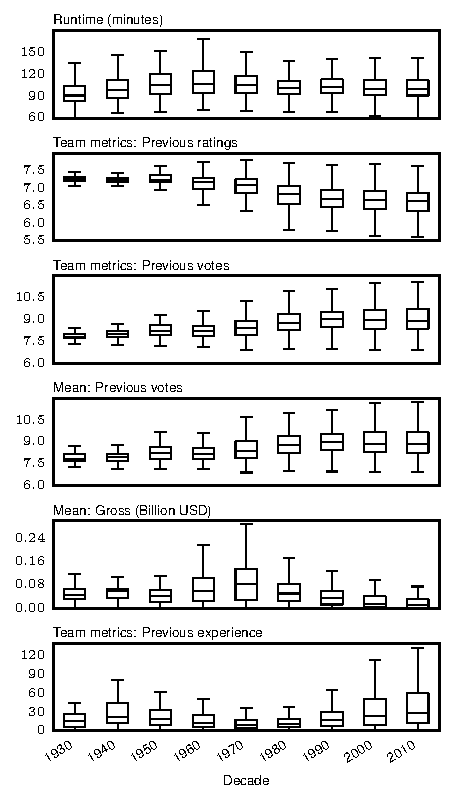
\includegraphics[width=0.7\columnwidth,height=18cm]{../../images/features_dist_ntop.pdf}
\caption{\label{fig:features_dist_ntop}Distribution of non-topological features
throughout the years.}
\end{center}\end{figure}

\section{Feature Characterization}
\label{sec:feature_char}
We present distributions from the selected features across the decades in
Figures~\ref{fig:features_dist_ntop}~and~\ref{fig:features_dist_top}. Features
have very different distributions throughout the years, indicating that the
movie producing network is dynamic and constantly evolving, albeit in a slow
pace\footnote{Figures~\ref{fig:hist_feat_ntop}~and~\ref{fig:hist_feat_top}
(presented in detail in Chapter~\ref{chapter:analysis}) present the
distribution of selected features in the whole set of data, but in the form of
color-coded histogram bars according to the movies performance group.}

\begin{figure}[!htb]\begin{center}
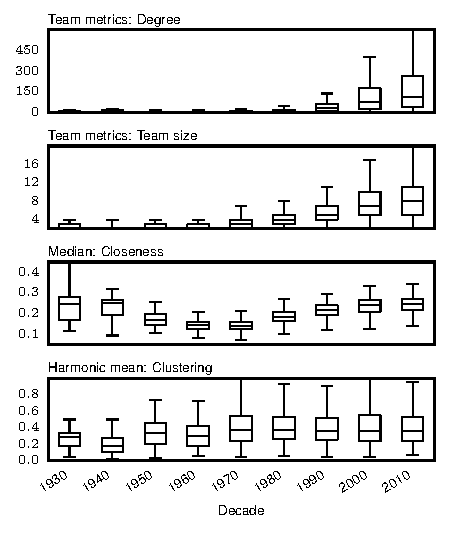
\includegraphics[width=0.78\columnwidth]{../../images/features_dist_top.pdf}
\caption{\label{fig:features_dist_top}Distribution of topological features
throughout the years.}
\end{center}\end{figure}

\begin{figure}[!htb]\begin{center}
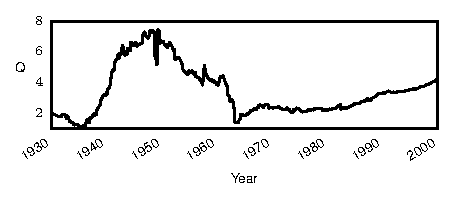
\includegraphics[width=0.78\columnwidth]{../../images/plot_q_1k.pdf}
\caption{\label{fig:q}Evolution of the small world coefficient for the IMDb network
cut considered in this research.}
\end{center}\end{figure}

We can see from these characterizations that different performance groups have
different distributions for the features being extracted. This is an important
indicator that the extracted features can indeed provide information on movie
performance.

Analyzing the features and their distributions also yields interesting insights
into the network. Figure~\ref{fig:q} shows the evolution of the small world
coefficient from the whole graph thorough the years. We can see a clear
disruption in the organization of the network in the 40s and 50s, that was
probably caused by World War II.\@ The efforts on the war and infrastructural
recovery that followed it could have captured resources that were previously
available for movie production. Also, the war destruction could have taken away
many filming sets, equipments, and even lives of actors and producers.

We observe that the post-war rise in the network's small world coefficient was
not as intense as in pre-war years. We hypothesise that this reflects a greater
division of the world, as movies producers from opposing cold war countries
would not be able to cooperate. Also, during the Cold War, producers and
directors (mostly in the USA) were persecuted as communists, that lead to a
decrease in production. Moreover, in recent years the cost of movie
production went down, what could have resulted in a greater pool of movie
producers spread around the world, leading to the existence of more teams that
are not closely knit in a central core.
  % this is how we define features from teams
\section{Feature Interaction}
\label{sec:feature_interac}
The interaction between features must also be considered: for instance, even if
a feature is seemingly unrelated to the target variable, when seen in
combination with other features, patterns may emerge. In order to study the
interaction among features, we created movie scatter plots where dot colors are
set according to movie performance groups, and axes represent features'
normalized values.

Specifically, Figure~\ref{fig:interaction} shows the formation of colored
clusters. The colors encode team's performance, which indicates that certain
combination of features can be used to help identifying team's performance. To
take advantage of this phenomena, we also included the product of every feature
pair as new features. There are dozens of possible pairs such that analysing
every pair individually is not practical. Machine Learning techniques are
employed to automatically identify pairs that add the most relevant
information. Figure~\ref{fig:interaction} presents some of the relevant pairs
for illustrative purposes.

There are two ways to calculate feature interaction: normalizing the features
to the [0--1] interval (using a simple linear interpolation) and then
calculating their product, or doing the same in reverse order. From
experimental evaluation, both methods produce similar results, but normalizing
before calculating the product performs slighting better. We assume this
happens because multiplying variables of the same magnitude mimics better the
way in which variables interact.

\begin{figure}[t]\begin{center}
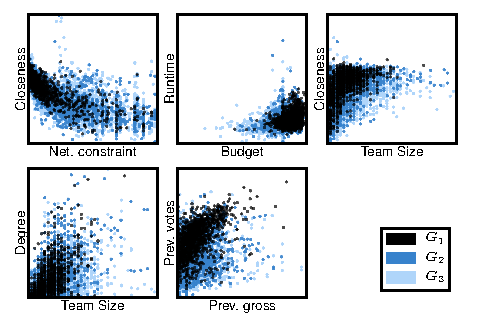
\includegraphics[width=\columnwidth]{../../images/feature_interaction.pdf}
\caption{\label{fig:interaction}Joint scatter plot of movies per features. The
shade of a point represents its performance group. Dark clusters form 
in the graph, meaning iteration between features should be considered.}
\end{center}\end{figure}
  % this is how we define features from teams
\section{Movie Success Prediction Model}
\label{sec:model:prediction}
In this section, we present the regression model chosen for experimentation
and provide a general overview of the proposed prediction model.

The movie success prediction task can be formally defined as follows. Consider
the set of movies $\mathbb{M}$ as the feature length movies for cinema with at
least one producer connected to the giant component (as defined in
Section~\ref{sec:filter}). Each movie $m \in \mathbb{M}$ has a set of features
$\mathbb{F}$, and each feature $f \in \mathbb{F}$ provides information about
$m$. For each success parameter (gross, votes and rating), the problem lies in
adjusting all $k$ coefficients of a linear combination of all $f$ features in
such way that this linear combination best fits the success parameter being
modeled considering all movies in $\mathbb{M}$. Such fitting of coefficients is
performed by a regression model, which estimates the relationship between the
features and each parameter.

Overall, we consider a set of 121 features spanned over three main aspects of
movies: characteristics of a motion picture itself, topological characteristics
from its production team, and the team's past success and experience
(Section~\ref{sec:features}). As for~\cite{Ghiassi2015}, our model only uses
features available \textit{before} the movie release and thus may be used to
make predictions (see Algorithm~\ref{algo:predictor} in
Chapter~\ref{chapter:analysis})

We rely on a multivariate Bayesian Ridge regression model to predict each movie
success parameters described in Section~\ref{sec:success}. This is a linear
regression model that uses Bayesian Inference and is similar to the Ridge
regression model. This regression model is well described in the literature
(Chapter~\ref{chapter:fundamentals}). It was chosen because it better handles
features with lots of noise (i.e., considerable unexplained variation is
observed when modeling the data). Two other regression algorithms were also
tried: the Support Vector Regression (SVR) and the Ordinary Least Squares (OLS,
Section~\ref{sec:ml}). However, comparing the resulting coefficients of
determination ($R^2$) shows the Bayesian Ridge regression model outperforms
them both.

Most linear regression techniques, including the one used in this study, work
best when their input features and target features are normalized and scaled to
the same magnitude. Therefore, all of our features are normalized, as well as
our target variables. There are two major techniques to achieve this. The first
is scaling the values to fit within the [0, 1] interval. The second is to
transform the data so that its mean equals zero and variance equals one.  Both
normalization techniques were attempted, and zero-one scaling provided better
results.
  % and this is how we predict team success
